\documentclass{beamer}

\usepackage{beamertheme Frankfurt}
\usepackage{beameroutertheme miniframes}
\usepackage{beamerinnertheme rounded}
\usepackage{beamercolortheme seahorse}
\usepackage{beamerfonttheme professionalfonts}

\usepackage[utf8]{inputenc}
\usepackage[T1]{fontenc}
\usepackage[ngerman]{babel}

\usepackage{csquotes}
\usepackage{color}
\usepackage{textcomp}
\usepackage{bookmark}
\usepackage{graphics}
\usepackage{listings}
\usepackage{lmodern}
\usepackage{marvosym}
\usepackage{microtype}
\usepackage{url}

\title{JumpVM}
\subtitle{Das neue Tool für die Compilerbau I + II Übungen}
\author{Tim Wiederhake}
\institute{Institut für Programmiermethodik und Compilerbau}
\date{04.11.2014}

\setbeamertemplate{footline}[frame number]

\lstset{
	language={Java},
	basicstyle={\scriptsize\ttfamily},
	breaklines={true},
	escapechar={§},
	moredelim={**[is][\color{red}]{@}{@}}
}

\AtBeginSection[]{
	\begin{frame}
		\tableofcontents[currentsection]
	\end{frame}
}

\begin{document}
\begin{frame}
	\maketitle
\end{frame}

\begin{abstract}
	Die \enquote{Java Unified Multi Paradigm Virtual Machine} (JumpVM) ist das 
	neue Übungswerkzeug für die Vorlesungen \enquote{Einführung in den 
	Übersetzerbau} und \enquote{Übersetzung fortgeschrittener Sprachkonzepte} 
	und löst die bisherigen Werkzeuge \enquote{pmach}, \enquote{wim} und 
	\enquote{mama} ab.
	
	In diesem Vortrag werden die Schwächen der bisher genutzten Werkzeuge 
	gezeigt, die Erweiterungen der JumpVM gegenüber diesen Werkzeugen 
	vorgestellt und die grundlegende Verwendung der JumpVM erläutert.
\end{abstract}

\begin{frame}
	\tableofcontents
\end{frame}

\section{Bestandsaufnahme}
\subsection*{Über mich}
\begin{frame}{Über mich}
	\begin{itemize}
	\item Informatik-Student (Master) der Universität Ulm
	\item Vorlesungen Compilerbau I + II gehört
	\item JumpVM entsteht als Projektmodul
	\end{itemize}
\end{frame}

\subsection*{Inhalt}
\begin{frame}{Inhalt der Vorlesungen}
	Übersetzerbau für
	\begin{itemize}
	\item Imperative Sprachen (Pascal)
	\item Funktionale Sprachen (Haskell)
	\item Logische Sprachen (Prolog)
	\item Objektorientierte Sprachen (C++)
	\end{itemize}
\end{frame}

\subsection*{Inhalt}
\begin{frame}{Inhalt der Übungen}
	\begin{itemize}
	\item Vertiefen
	\item Anwenden
	\item Üben
	\end{itemize}
	
	\visible<2->{\alert{$\Rightarrow$ JumpVM}}
\end{frame}

\subsection*{Die bisherigen Werkzeuge}
\begin{frame}{MaMa, Pmach und Wim}
	\begin{itemize}
	\item Geschrieben in Gofer
	\item Grafische Oberfläche mit Tcl / Tk
	\item Entstanden 1995 -- 1998
	\item Installiert in den Linux-Rechnerpools der SGI unter 
	\texttt{/opt/Abteilungen/pm/Gofer\_VM/bin}.
	\end{itemize}
\end{frame}

\begin{frame}[plain]
	\centering
	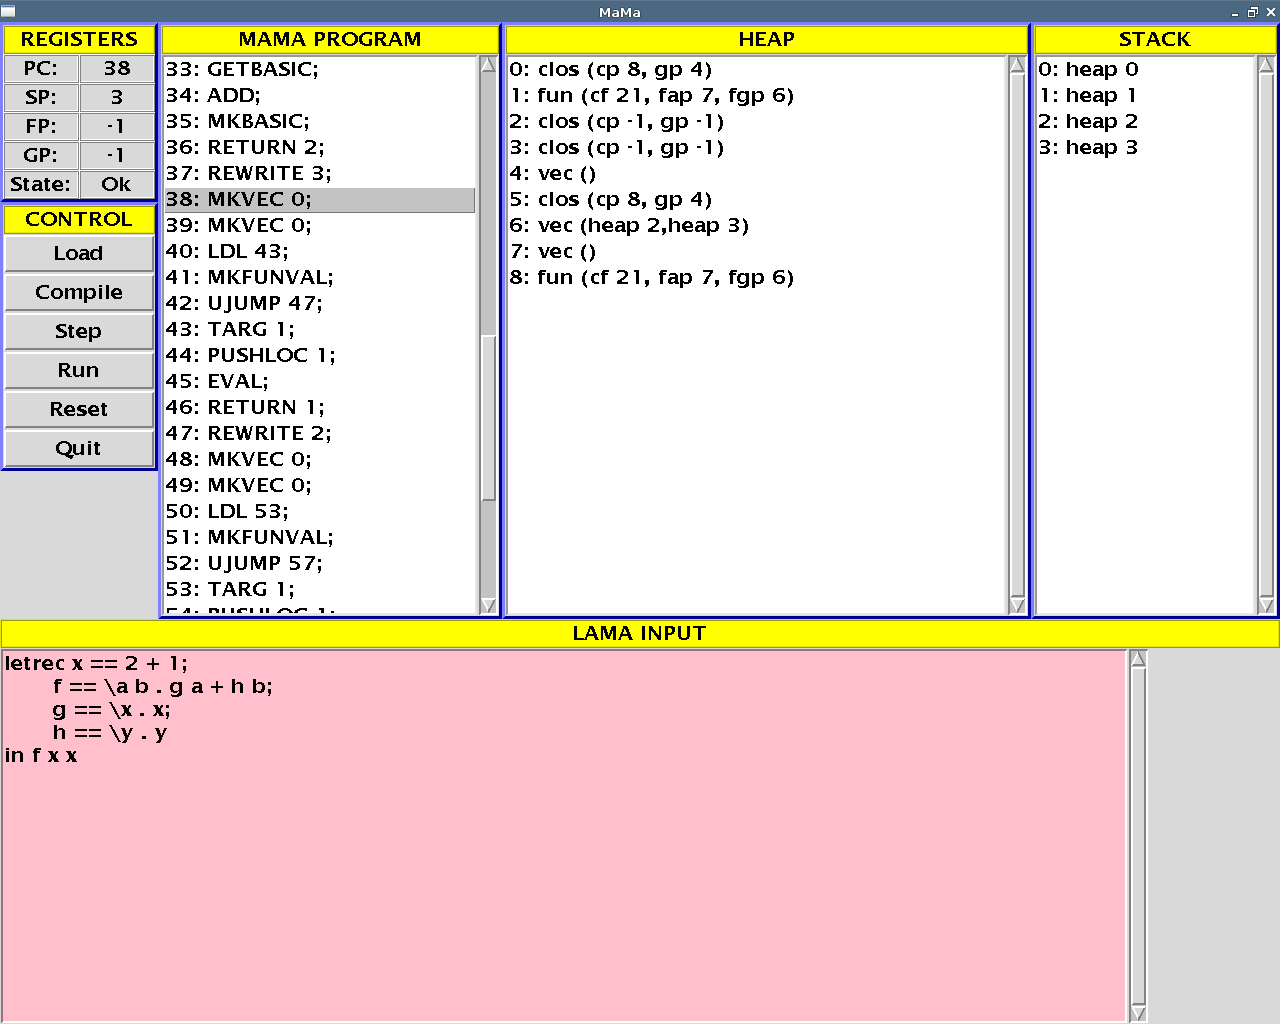
\includegraphics[width=\textwidth]{screenshot_old_mama.png}
\end{frame}

\begin{frame}[plain]
	\centering
	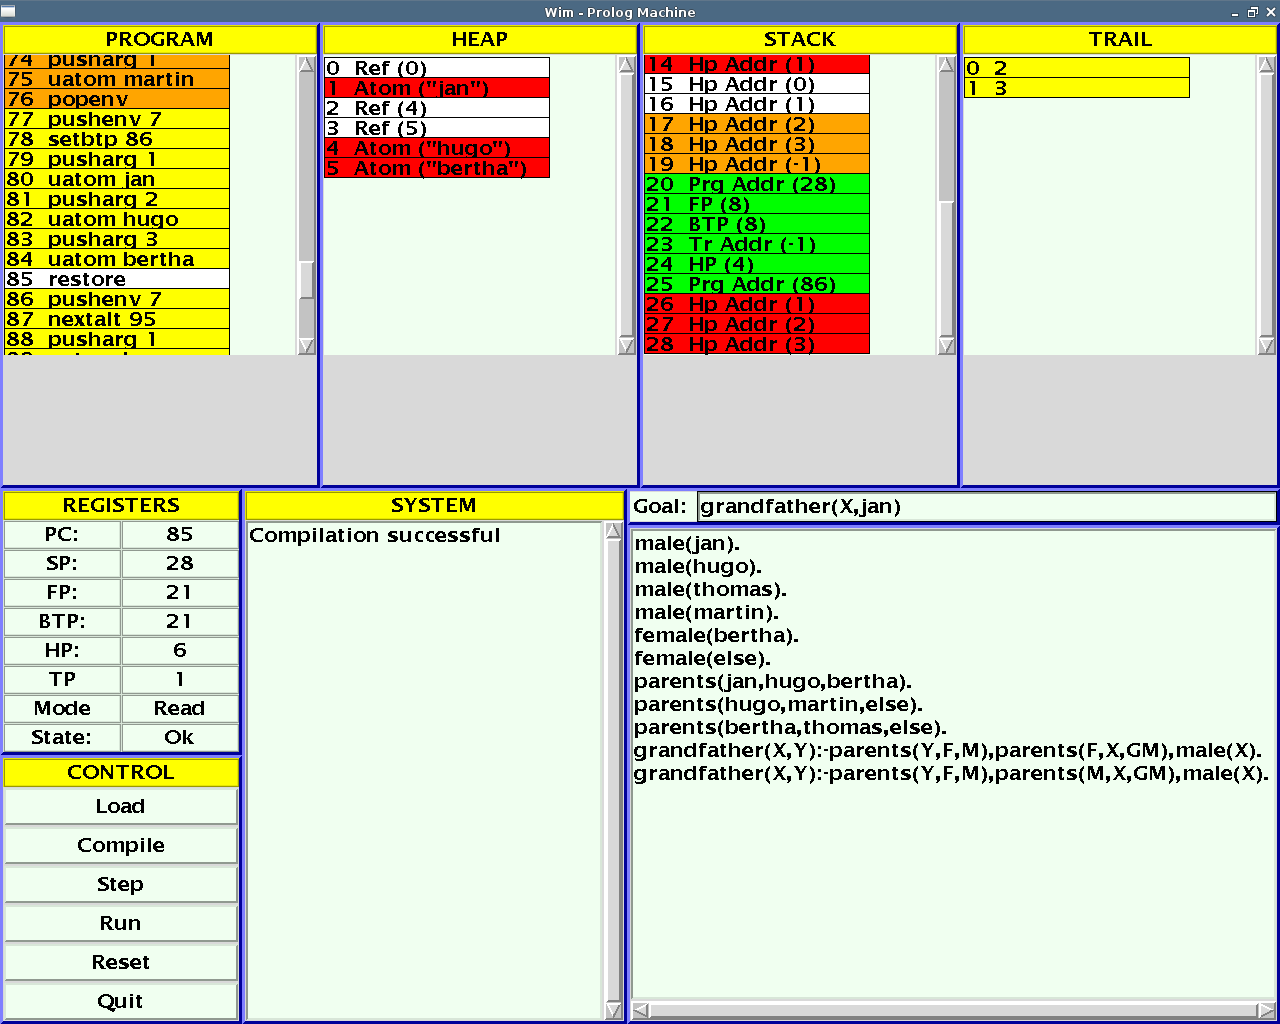
\includegraphics[width=\textwidth]{screenshot_old_wim.png}
\end{frame}

\begin{frame}[plain]
	\centering
	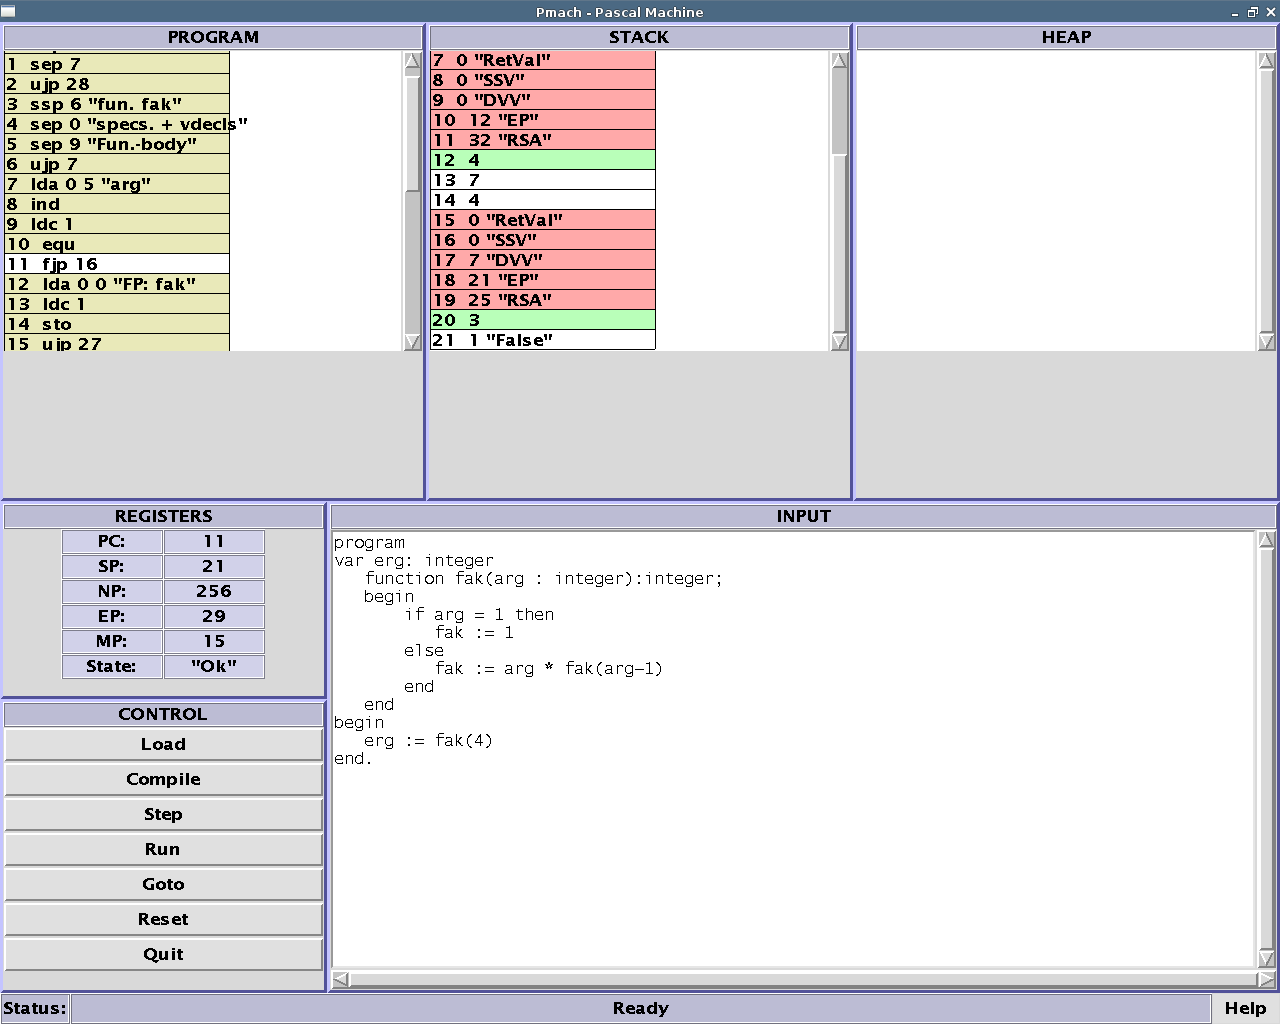
\includegraphics[width=\textwidth]{screenshot_old_pmach.png}
\end{frame}

\section{Defizite}
\subsection*{Defizite}
\begin{frame}[fragile]{Wart- und Erweiterbarkeit}
	\begin{block}{Gofer (Haskell-Dialekt, \textdied 1994)}
	\begin{lstlisting}[language=Haskell]
dostep :: Status -> Edit -> GUI ()
dostep s ou = do
  (m@(rg@(pc',_,_,_,_,_,_),he,st,tr,err),p) <- readGVar s
  if length p == 0
    then do writeGVar s ((rg,he,st,tr,Stopped),p)
            sysout ou "No Program"
    else
    if (err /= Ok) || (pc' >= length p)
      then do writeGVar s ((rg,he,st,tr,Stopped),p)
              tk_showError "You must reset the machine first"
      else do if ((fst.fst) (p !! pc')) == "halt"
                then sysout ou (varstr st he)
                else done
              let m'@(_,_,_,_,err') = step (snd (p !! pc'))
                                            (incpc m)
(...)
	\end{lstlisting}
	\end{block}
\end{frame}

\begin{frame}{Installierbarkeit}
	\begin{itemize}
	\item Nur in den Linux-Pools der SGI
	\item Keine Windows- oder Mac-Versionen
	\item Abhängigkeiten (Tk 4.2 $\rightarrow$ 8.6 in Debian Jessie)
	\item Eigene Gofer/Tk-Bindings
	\item Unbekannte Lizenzierung
	\item WiSe 2014: Umstellung des Linux-Pools auf Fedora:
		Nicht mehr ausführbar
	\end{itemize}
\end{frame}

\begin{frame}{Benutzerfreundlichkeit}
	\begin{itemize}
	\item Uneinheitliche GUI (Register, Speicher, Buttons)
	\item Stürzt ohne Fehlermeldung bei falscher Syntax ab
	\item Bugs in \enquote{wim} ($\rightarrow$ \enquote{\texttt{equals(a, b)}})
	\item Bugs in \enquote{PMach} ($\rightarrow$ \enquote{\texttt{true = false = 0}})
	\item Gofer-Interpreter stürzt bei größeren Programmen ab
	\item Ausführung verlangsamt sich mit jeder Instruktion
	\end{itemize}
\end{frame}

\section{JumpVM}
\subsection*{}
\begin{frame}{Ziele}
	\begin{itemize}
	\item<2-> Plattformunabhängigkeit
	\item<2-> Populäre Programmiersprache
	\hfill{} \visible<3->{$\Rightarrow$ Java}
	\item<4-> Vereinheitlichung der Oberfläche
	\item<4-> Generalisierung von Code
	\hfill{} \visible<5->{$\Rightarrow$ JumpVM-\enquote{Framework}}
	\item<6-> Einhalten von Standards
	\hfill{} \visible<7->{$\Rightarrow$ Checkstyle}
	\item<8-> Ausführliche Dokumentation
	\hfill{} \visible<9->{$\Rightarrow$ JavaDoc + \LaTeX{}}
	\item<10-> Tests!
	\hfill{} \visible<11->{$\Rightarrow$ JUnit}
	\item<12-> Eindeutige Lizenzierung
	\hfill{} \visible<13->{$\Rightarrow$ Gnu GPL 3+}
	\item[$\Rightarrow$]<14-> \enquote{Paretodominante} Lösung
	\end{itemize}
\end{frame}

\subsection*{Screenshot}
\begin{frame}[plain]
	\centering
	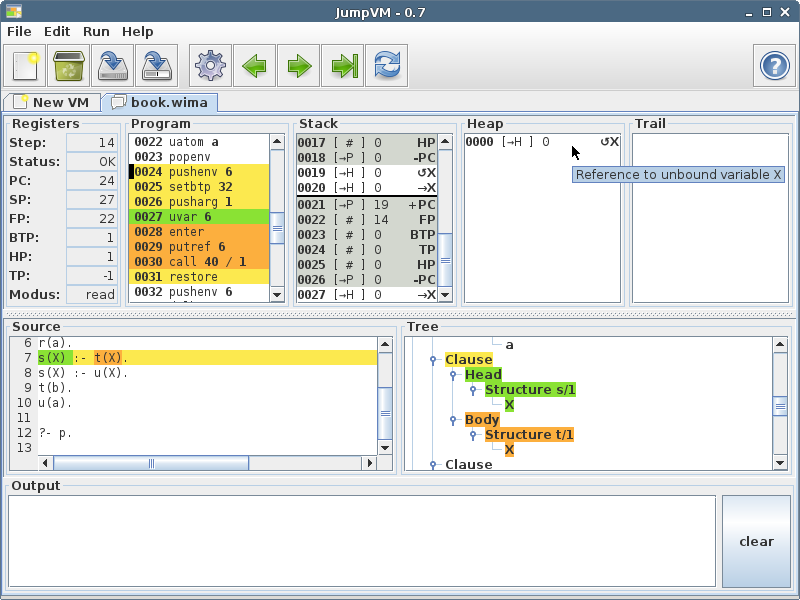
\includegraphics[width=\textwidth]{screenshot.png}
\end{frame}

\subsection*{}
\begin{frame}{Fähigkeiten}
	\begin{itemize}
	\item<2->Vollständiger Funktionsumfang der \enquote{PMach}, \enquote{wim}
		und \enquote{mama}
	\item<3-> Brainfuck-Compiler als Beispiel für die Verwendung des 
		JumpVM-Frameworks
	\item<4->Fehlermeldungen, Hilfetexte
	\item<5-> Erweiterte Beispiele
	\item<6-> Anzeige und Export des Syntaxbaumes und der Maschinenbefehle
	\end{itemize}
\end{frame}

\begin{frame}{Fähigkeiten (forts.)}
	\begin{itemize}
	\item<1-> Ändern von Registerinhalten, Ändern des Speicherinhaltes
	\item<2-> Durchgehende Annotation und Typisierung von Werten
	\item<3-> Schrittweises Rückgängigmachen der Ausführung
	\item<4-> Abbildung Sourcecode $\leftrightarrow$ Syntaxbaum $\leftrightarrow$ 
		Maschinenbefehle
	\item<5-> Befehle für Eingabe und Ausgabe
	\end{itemize}
\end{frame}

\section{Demonstration}
\begin{frame}{Demonstration}
	\vfill{}
	\begin{block}{Bezugsquelle}
		\href{https://github.com/twied/jumpvm/releases}
		{\texttt{https://github.com/twied/jumpvm/releases}}
		\ComputerMouse{}
		
		\hfill{} \ldots{} und bald\texttrademark{} im Linux-Pool vorinstalliert.
	\end{block}
	\vfill{}
	\begin{alertblock}{Danke für Ihre Zeit!}
	\end{alertblock}
	\vfill{}
\end{frame}
\end{document}
